% !TEX root =  ./main.tex

\subsection{Comorbidity Treatment Analysis}

%The paper~\cite{DBLP:conf/cmsb/BowlesBBFGM24} introduced the notion of RS with guarded contexts, recalled in \Cref{sec:RS}.
%to model scenarios where the entities to be provided by the context are dependent upon the current state, which is a common situation arising, e.g., in drug administration and \emph{in silico} experiments. 
This case was studied in~\cite{DBLP:conf/cmsb/BowlesBBFGM24}, where it was used as motivation for the introduction of RS with guarded contexts, recalled in \Cref{sec:RS}. It concerns the risk reduction of medication harm in the treatment of patients with comorbidities; i.e., patients with two or more long-term chronic conditions (such as diabetes, hypertension, cardiovascular diseases, chronic kidney disease, cancer, chronic obstructive pulmonary disease, among many others), who are therefore subject to follow several treatment plans simultaneously, called \emph{clinical guidelines}~\cite{feder1999using,woolf1999potential}. Since clinical guidelines address a single disease, comorbidities easily lead to  \emph{polypharmacy}, where 5 or more medications must be administered, increasing the risk of adverse drug reactions, or of making certain drugs less effective when combined~\cite{Gut12}. Using formal methods for risk mitigation intends to help doctors choose between alternative treatment options as well as to point out missing conditions that could be helpful to revise and update clinical guidelines. 

\subparagraph*{Features of interest.}
In this case study, reachability and causal analysis are key issues.
Specifically, reachability is used to address questions such as \emph{can the combination of clinical guidelines expose the patient at serious risks because of drugs interference?}
Then, in the affirmative case, causal analysis can help to detect which medical decisions would be directly responsible for causing serious harm as well as to point out  which alternative treatment would be available, if any.
We have selected this case study because the use of guarded contexts poses new challenges in terms of causal analysis: an external choice, apparently made by the context, might in fact be the only option available given the actual state of the system. \todo{A: I don't quite get it - what is the new challenge?}

\subparagraph*{Experimental set up.}
The RS encoding proposed in~\cite{DBLP:conf/cmsb/BowlesBBFGM24} relies on a formal representation of patient profiles, medical guidelines and adverse drug reactions.

For medical guidelines, it takes in input the event structure modelling of therapies introduced in~\cite{BC17c}. Roughly, to each event $e$ there is an identifier $\mathsf{E}_e$ defined as a sum of processes, one for each outgoing arc of $e$. If some guard is attached to the arc, then the corresponding alternative is also guarded. When some drug prescription for $d$ is present in a node, then the corresponding choice produces $\mathsf{get}\_d$. Similarly, if the therapy requires stopping some drug $d$, the entity $\mathsf{stop}\_d$ is produced.
Concurrent events are activated separately.\todo{This sentence is not clear to me.}

The patient profile is determined by the conditions that trigger the treatment (e.g., headache, hypertension) and by the conditions that appear in the arc labels of the event structure (e.g., pregnant, asthma). We call them \emph{features}. The patient profile is thus just a combination of features. Correspondingly, there is one context $\mathsf{K}_f = \emptyset.\mathsf{Empty} + \{f\}.\mathsf{Empty}$ for each feature $f$, and any possible combination of features is accounted for by their parallel composition $\prod_f \mathsf{K}_f$. Alternatively, specific profiles can be investigated by removing some alternatives from each $\mathsf{K}_f$.\todo{Why is this useful?}
Once the profile is determined by the context, it is preserved during the rest of the computation by reactions of the form $(\{f\},\emptyset,\{f\})$, one for each feature.

For each drug $d$ that appears in the therapies, we consider three corresponding entities $\mathsf{get}\_d$, $\mathsf{stop}\_d$  and $d$: the first represents the prescription of $d$ by the doctor, the second the removal of $d$ from the current treatment and the third the intake of the drug by the patient. 
Entities $\mathsf{get}\_d$ and $\mathsf{stop}\_d$ will be provided by the context that models the guideline, as discussed above. 
For each drug, $d$ there will be the following reactions: $(\{\mathsf{get}\_d\},\{\mathsf{stop}\_d,\mathsf{stop}\_c\},\{d,c\})$ modelling the intake of the drug $d$ as for doctor prescription, and $(\{d\},\{\mathsf{stop}\_d,\mathsf{stop}\_c\},\{d,c\})$ modelling the prosecution of the therapy.\todo{What is $c$ here?}
Adverse drug reactions are provided in the form of so-called ADR tables.
Each row corresponds to a set of medications $M$, a textual description of their side effects and risks when used in combination, and a severity level $m$ (e.g., minor, moderate, major).
Each row translates to a reaction $(M,\emptyset,\{m\})$. 

\subparagraph*{Analysis goals.}
The goal of the analysis is to explore the combination of clinical guidelines in the presence of comorbidities and for different patient profiles to detect if major risks can arise from the treatments and which profiles are exposed at severe risks.\todo{This reads like a duplication}

\subparagraph*{Previous approach.}
The approach outlined in~\cite{DBLP:conf/cmsb/BowlesBBFGM24} has been used to synthesize the patient profiles that are more at risk, as a support for dynamic guideline revision: by refining guarded contexts to prevent severe effects for specific patients, we can readily check the efficacy of the changes.

\subparagraph*{GROOVE experimentation.}

The benefit of using GROOVE in this case study is that, besides identifying situations where a risk is found, the corresponding occurrence graph can be easily generated, using the process outlined in \Cref{sec:RS2GTS}. This provides a means to medical experts to more easily analyze root causes: for any risk that has been identified, what is the causal structure of the steps and entities leading up to it?

GROOVE can be used for full state space generation, for instance to count the number of ways a minor, moderate or major risk can arise. Some statistics are:

\begin{center}
\begin{tabular}{lrr}
\bf Measurement & \bf States & \bf Time (s) \\
\hline
Total states   & 309.798 & 2.464 \\
Major risks    &  91.113 & 2.447 \\
Moderate risks &  97.805 & 1.534 \\
Minor risks    &      24 & 2.218
\end{tabular}
\end{center}

At first sight, the number of major (and moderate) risks seems impossibly large, and evidently implies that there are patient profiles that give rise to many risks. However, this should be interpreted with care: the count refers to the total configurations, and there may very well be entities whose presence or absence does not causally contribute to a risk (essentially because they do not occur in its occurrence graph). Thus, configurations counted as separate risks may well reduce to the same causation. To analyse this further, one would have to construct (and prune) the occurrence graphs for all risk configurations, and compare them on that basis. Though this is beyond the scope of this paper, such an analysis is in principle straightforward to carry out in \GROOVE --- it is a matter of combining the three steps in \Cref{fig:chain} into a single rule system.
 
\medskip\noindent By exploring only up to a certain depth, we can get some idea of the number of steps after which a risk typically appears, which in turn indicates the complexity of the context in which it appears. For instance, the following table shows how many major risks occur after a fixed number of reaction steps.

\begin{center}
\begin{tabular}{lrr}
\bf Steps & \bf Risks & Time (s) \\
\hline
3 &       0 &    3 \\
4 &     716 &    8 \\
5 &  10.033 &  158 \\
6 &  45.932 &  390 \\
7 & 119.932 & 1241 \\
\end{tabular}
\end{center}

Note that the results (in terms of number of risks found) are not entirely comparable to those in the first table, since by explicitly counting the length of the trace we lose the ability to identify cyclic behaviour; hence if the same configuration (in terms of entities present) can reoccur after (say) 4 and 6 steps, then any major risk directly derived from that configuration will be counted twice, after 5 and 7 steps, respectively.

\medskip\noindent Alternatively, we can stop exploring after having found a predetermined number of risks. By setting the exploration strategy to breadth-first search, it is guaranteed that the risks found are those reached after the shortest number of steps, meaning they are the easiest to analyze visually. For instance, \Cref{fig:cmsb-pruned} shows the occurrence graph of the first major risk found in this way.

\begin{figure}
\centering
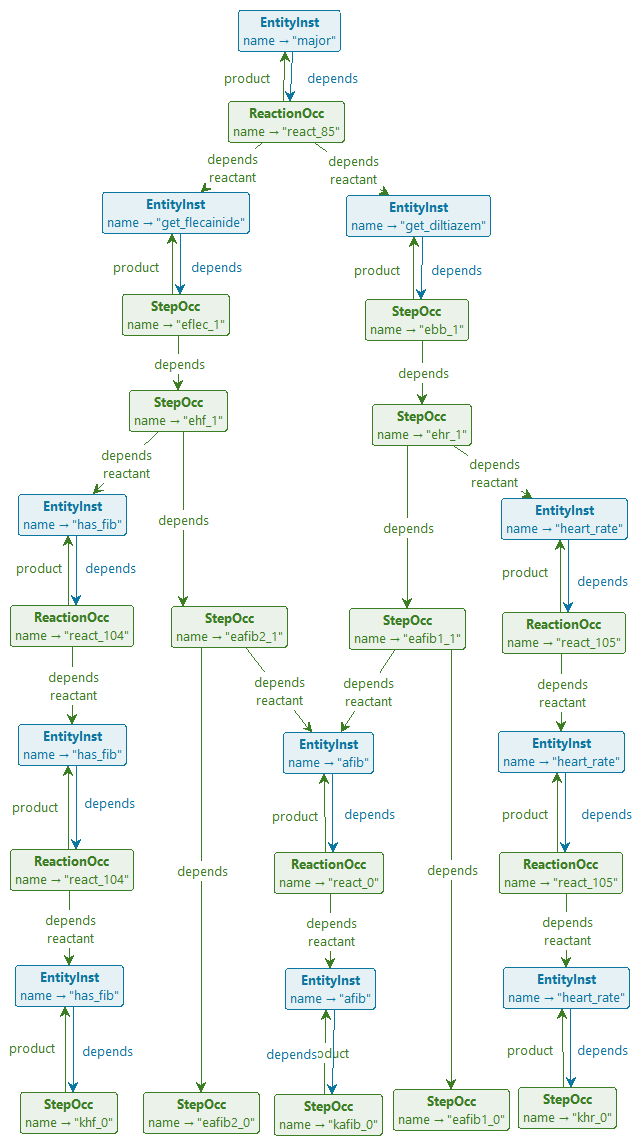
\includegraphics[scale=.3]{./figs/cmsb-pruned}
\caption{Occurrence graph of a major risk.}
\label{fig:cmsb-pruned}
\end{figure}

The patient configuration in question is a combination of ``has\_fib'', ``afib'' and ``heart\_rate''; the combination of the first two leads to the prescription of fleacinide and the second to the prescription of diltiazem, the combination of which should, however, be avoided. By counting the longest chain of \StepOcc-nodes, it is confirmed that it indeed takes 4 steps to establish this risk.

\medskip\noindent Compared to the prior results in \cite{DBLP:conf/cmsb/BowlesBBFGM24}, the advantages of using \GROOVE lie in performance and flexibility:
\begin{itemize}
\item The time needed to analyze the entire state space is around 41 minutes \GROOVE; while not particularly fast, this still compares very favourable to the 5 hours needed by \BioResolve.

\item Finding shortest paths to risk configurations and computing occurrence graphs is part of the core functionality of \GROOVE --- given, of course, suitable rule systems that encode the chosen notion of causal dependency.
\end{itemize}

